\documentclass[tikz, border = 1 cm]{standalone}
\usepackage{tikz}

\usepackage{tkz-euclide}

\begin{document}
    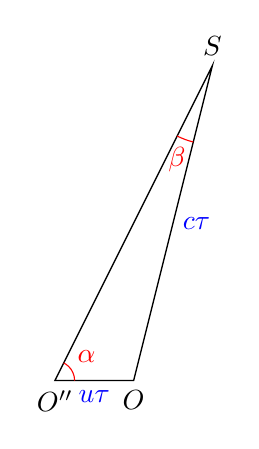
\begin{tikzpicture}
      \tkzDefPoint(0,0){O1}
      \tkzDefPoint(1,0){O2}
      \tkzDefPoint(2,4){S}

      \draw [line width=0.5pt] (O1) -- (O2) -- (S) -- cycle;

      \begin{scope}
        \clip (O1) -- (O2) -- (S) -- cycle;
        
         \draw [red] (O1) circle (0.25);
        \draw [red] (S) circle (1);
      \end{scope}

      \node[red] at (0.4,0.3) {$\alpha$};
      \node[red] at (1.55,2.8) {$\beta$};

      \node[below] at (O1) {$O''$};
      \node[below] at (O2) {$O$};
      \node[above] at (S) {$S$};
      \node[right,blue] at (1.5,2) {$c\tau$};
      \node[below,blue] at (0.5,0) {$u\tau$};
    \end{tikzpicture}
\end{document}
